\documentclass[a4paper,10pt]{article}

\usepackage{kotex}
\usepackage{datetime}
\usepackage{fullpage}
\usepackage{indentfirst}
\usepackage{amsmath}
\usepackage{amsfonts}
\usepackage{amssymb}
\usepackage{bm}
\usepackage{enumerate}
\usepackage{listings}
\usepackage{graphicx}
\usepackage{float}
\usepackage{multirow}

\newdateformat{koreandate}{\THEYEAR년 \twodigit{\THEMONTH}월 \twodigit{\THEDAY}일}
\renewcommand{\abstractname}{초록}
\renewcommand{\contentsname}{목차}
\renewcommand{\figurename}{그림}
\renewcommand{\tablename}{표}
\graphicspath{ {images/} }

\linespread{1.5}

\begin{document}

\title{뉴스 기사를 이용한 주식 가격의 변동 예측}
\author{
  서울대학교 컴퓨터공학부 \\
  2009-11744 심규민
}
\date{\koreandate\today}
\maketitle

\begin{abstract}
TODO
\end{abstract}

\tableofcontents

\thispagestyle{empty}
\pagebreak
\setcounter{page}{1}

\section{서론}

\subsection{연구 목적}

본 연구에서는 우리나라 주식 시장에 상장한 회사들에 관한 인터넷 뉴스 기사를 통해 그 회사들의 주가가 단기적으로 어떻게 변동할지 예측해보았다.
효율적 시장 가설(Efficient Market Hypothesis)에 따르면 주식 시장에는 수많은 요인이 반영되어 있기 때문에, 주가는 예측할 수 없게 움직인다.
주식 분석 방법 중 기본적 분석(Fundamental Analysis) 방법에 의하면 주가가 변동하는 요인은 회사의 실적, 전망 등 다양하다.
이러한 요인들에 대한 소식은 입소문, 뉴스를 통해 전달되지만, ``소문에 사고 뉴스에 팔아라''는 말이 있는 것처럼 뉴스는 주가보다 늦게 반응한다는 것이 중론이다.
그런데 Gidofalvi et al.의 연구에서 뉴스 기사로부터, 그 예측력은 낮지만 효율적 시장 가설에 반하는, 주가 변동의 예측이 가능함을 보여주었다.
본 연구는 이 선행 연구를 검증하는 목적으로 NASDAQ 시장이 아닌 국내 시장에 적용하여 보고자 하였다.
또한 선행 연구에서는 주가의 움직임을 예측할 때 나이브 베이즈 분류기(Naive Bayes Classifier)를 사용하였는데,
본 연구에서는 이것을, 최근 기계학습(Machine Learning) 분야에서 주목받고 있는, 인공신경망(Artificial Neural Network)으로 대체해보았다.

\subsection{선행 연구 분석}

선행 연구(Gidofalvi et al. 2001)는 다음과 같이 크게 네가지 단계로 이루어졌다.
\begin{enumerate}
\item 주가 데이터 수집
\item 주가에 따른 뉴스 기사의 정렬(alignment), 점수화(scoring), 분류(labelling)
\item 나이브 베이즈 분류기 학습(training)
\item 분류기 평가(evaluation)
\end{enumerate}
먼저, 특정 종목(회사)에 대해 시간별 주가 데이터를 수집한다.
그리고 나서 그 종목 뉴스 각각에 대해 정렬, 점수화, 분류 과정을 거친다.
정렬 과정에서는 임의의 시간 간격을 정해서 해당 뉴스가 공개된 시각을 기준으로 그 전 몇 분과 그 후 몇 분을 그 뉴스가 영향을 주는 범위로 보는 것이다.
예를 들어 $[-20, 30]$ 시간 간격에 대해, 어떤 뉴스가 오전 10시 30분에 공개 되었다면, 이 뉴스가 주가에 영향을 주는 범위는 오전 10시 10분부터 11시 0분까지가 된다.
정렬 과정에서는 이 범위가 주식 시장이 열려 있는 동안만으로 한정하여 그 밖에 위치한 뉴스들을 걸러내는 작업도 한다.
점수화 과정은 뉴스가 영향을 주는 범위의 시작 시각과 끝나는 시각의 주가의 상대적 변화를 수치화 하는 과정이다.
구체적으로는 끝나는 주가를 시작 주가로 나누어 로그를 취한 값($\Delta price$)을 정규화 하여 사용한다.
정규화는 각 종목에 대한 $\Delta price$를 그 종목의 변동성($\beta$-값)으로 나누고, 주식 시장 index에 대한 $\Delta price$를 빼는 작업이다.
분류 과정은 점수화의 결과가 특정 threshold $\rho_{positive}$, $\rho_{negative}$에 대해
$\rho_{positive}$ 보다 크면 해당 뉴스에 의해 주가가 올랐다($UP$)고 표지하고,
$\rho_{negative}$ 보다 작으면 내렸다($DOWN$)고 표지하며,
그 사이일 경우 변하지 않았다($EXP$)고 표지하는 작업이다.
뉴스 기사의 분류 작업이 끝나면, 뉴스의 내용을 이루고 있는 각 단어들에 대한 나이브 베이즈를 가정하고 분류기를 학습 시킨다.
분류기의 입력은 뉴스 기사의 내용이며 출력은 분류 표지 ($UP, DOWN, EXP$) 중 하나이다.
마지막으로 이렇게 학습된 분류기를 이용하여, 최고의 성능을 갖는 정렬 시간 간격과 분류 threshold를 찾는다.

선행 연구의 결과는 논문 상에 정확한 정확도를 명시하지는 않았지만,
분류 threshold $\rho_{positive}=0.002$, $\rho_{negative}=-0.002$일 때 무작위 예측 보다 높은 성능을 보였고,
선행 연구 논문에서 제시한 그래프를 볼 때 그때의 $accuracy$는 약 $40\%$였다.
정렬 시간 간격은 $[-20,0]$과 $[0,20]$일 때 가장 의미 있는 성능을 내었으며,
$precision$과 $recall$은 각 표지별로 다르지만 $30\%$에서 $50\%$ 사이였다.

\section{데이터 수집}

본 연구를 위해, 선행 연구와 마찬가지로, 주가 데이터와 뉴스 기사 데이터를 수집하였다.
데이터를 가져올 종목은 KOSDAQ 시장에서 시가 총액 상위 30 종목 중 외국인 보유주 비율이 낮은(5\% 내외) 6개 종목으로 정했다.
그 이유는 첫째로 시가 총액이 큰 회사가 상대적으로 투자자들의 관심을 많이 받고 관련 뉴스가 많아서 인공 신경망을 학습 시킬 데이터를 많이 얻을 수 있다는 점이고,
둘째로는 KOSPI에 비해 주가가 낮은 KOSDAQ 종목 그리고 외국인 비율이 낮은 종목이 개인 투자자들의 거래 비율이 많을 것으로 예상되기 때문이다.
기관이나 외국인 등 투자 전문가들은 개인 투자자들에 비해 소식을 먼저 접하고 미리 움직일 가능성이 크다는 가정을 하였다.

\subsection{주가 데이터}

주가 데이터는 각 종목별로 날짜와 시각에 따른 주가의 리스트로 정의된다.
주가 데이터를 얻기 위해 국내의 한 증권사인 이베스트투자증권에서 제공하는 Xing API를 이용하였다.
Xing API의 COM(Component Object Model)을 사용하는 Windows Form 응용 프로그램을 C\# 언어로 구현하였다.
주가 데이터를 얻는 응용 프로그램의 전체적인 구조는 그림 \ref{fig:getting_price}와/과 같다.
\begin{figure}[h]
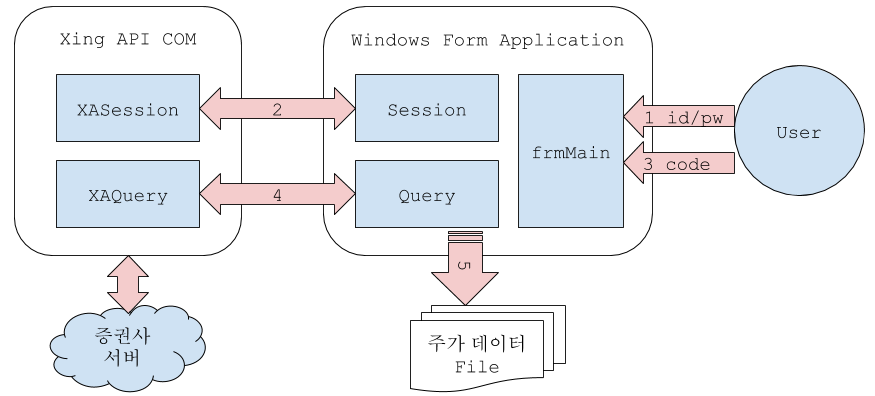
\includegraphics[width=\textwidth]{getting_price}
\centering
\caption{주가 데이터 수집 응용 프로그램의 구조}
\label{fig:getting_price}
\end{figure}
먼저 증권사의 API를 사용하기 위해 계정 아이디와 비밀번호, 공인인증서 비밀번호 등 사용자 정보를 받는다.
받은 사용자 정보를 Session 객체에 넘겨 COM 인터페이스를 통해 로그인 한다.
로그인이 완료되면 사용자가 주가를 조회하고 싶은 종목 코드를 입력한다.
마지막으로 주가를 조회하는 Query를 요청하여 주가 데이터를 얻고 이를 파일로 출력한다.
이렇게 수집한 주가 데이터는 뉴스 기사 데이터와 함께 인공 신경망을 구축하기 위해 사용되었다.
이를 위해서 주가 데이터 파일을 읽어서 단순히 데이터베이스에 옮겨 저장하는 스크립트를 작성하였다.
이 스크립트는 Python 언어로 작성하였으며 DBMS는 MongoDB를 사용하였다.
실제로 앞서 선택한 6개의 종목에 대해 Xing API로 한번에 가져올 수 있는 최대치인 약 1년치(2015년 6월 2일부터 2016년 5월 24일까지)의 10분 간격 주가 데이터를 얻었다.

\subsection{뉴스 기사 데이터}

뉴스 기사 데이터는 각 종목별로 날짜와 시각에 따른 뉴스 기사 본문의 리스트로 정의된다.
뉴스 기사는 네이버의 증권 서비스(m.stock.naver.com)에서 자동으로 수집하였다.
이 서비스에는 각종 신문사의 뉴스 기사를 한데 모아서 종목 이름이나 코드로 검색하여 볼 수 있는 기능이 있다.
그러나 이 서비스에서는 공식적으로 REST API를 제공하지 않기 때문에 이에 대한 레퍼런스 문서가 공개되어 있지 않다.
따라서 자동화 스크립트를 작성하기 위해 먼저 해당 서비스의 사이트를 분석하였다.
그림 \ref{fig:naver_stock}은/는 크롬 웹브라우져 개발자 도구로 해당 사이트를 분석하는 모습이다.
\begin{figure}[h]
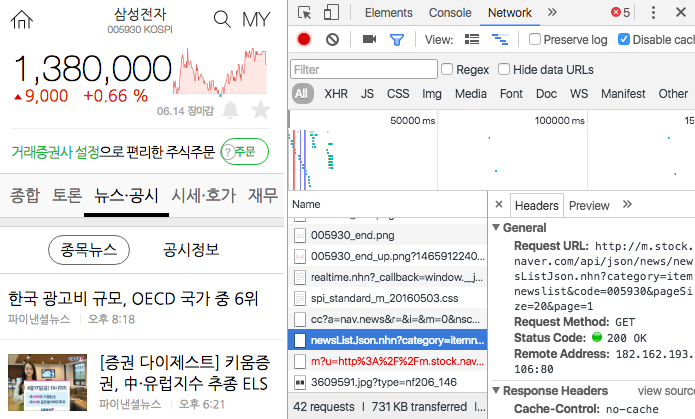
\includegraphics[width=0.8\textwidth]{naver_stock}
\centering
\caption{네이버 금융 서비스를 크롬 웹브라우져 개발자 도구로 분석하는 모습}
\label{fig:naver_stock}
\end{figure}
사이트 분석 결과 다음의 두 API end-point를 알 수 있었다.
\begin{itemize}
\item \texttt{GET /api/json/news/newsListJson.nhn?category=itemnewslist\&code=\&pageSize=\&page=}
\item \texttt{GET /api/html/item/itemNews.nhn?\&code=\&officeId=\&articleId=}
\end{itemize}
앞의 것은 종목 코드(\texttt{code})에 관련된 뉴스 기사들을 \texttt{pageSize}씩 나눴을 때 \texttt{page}번째에 해당하는 목록을 JSON 형식으로 돌려주는 API이다.
특정 회사의 종목 코드는 해당 서비스나 여러 증권사, 포털 사이트 등을 통해 쉽게 찾을 수 있다.
뒤의 것은 종목 코드(\texttt{code})와 신문사 아이디(\texttt{officeId}), 기사 아이디(\texttt{articleId})를 받아 해당 기사의 내용을 HTML 형식으로 돌려주는 API이다.
여기에 필요한 신문사 아이디와 기사 아이디는 목록 API 결과에 포함되어 있다.
자동화 스크립트는 Python 언어로 작성하였으며, 이를 통해 얻은 뉴스 기사 데이터는 인공 신경망 학습 코드를 간결하게 하기 위해 주가 데이터와 같이 MongoDB에 저장하였다.
Python의 \texttt{urllib} 라이브러리를 이용하여 REST 요청을 하고, \texttt{BeautifulSoup} 라이브러리를 이용하여 반환된 기사를 파싱하였다.
API에서 반환하는 기사는 제목, 내용, 광고 등이 섞여 있기 때문에 본문만 추출하고, 본문에도 내용과 상관없는 광고가 포함되어 있을 경우 제거해주었다.
실제로 앞서 선택한 6개의 종목에 대해 주가 데이터를 포괄할 수 있도록 현재(데이터 수집 당시 기준 5월 24일)보다 365일 이전의 기사까지 수집하였다.

\section{예측 모델}

\subsection{자연어 처리}

뉴스 본문
형태소 분석
KoNLPy
Mecab
명사

Feature 추출
bag of words
TF-IDF

\subsection{인공 신경망 학습}

MLP (Neural Net, softmax)

\section{결과 및 분석}

??

\section{결론}

인덱스 보정 (베타값)
topic modelling 뉴스 걸러내기

\section*{참고문헌}

\begin{enumerate}[ {[}1{]} ]
\item Gidofalvi, Gyozo, and Charles Elkan. ``Using news articles to predict stock price movements.'' \textit{Department of Computer Science and Engineering, University of California, San Diego} (2001).
\item 이베스트투자증권. ``XingAPI COM 개발 가이드'' \textit{http://etrade.co.kr/apiguide/guide.jsp?cno=200}.
\item 조대표. ``파이썬을 이용한 시스템 트레이딩 (기초편)'' \textit{https://wikidocs.net/book/110}.
\end{enumerate}

\end{document}
